\documentclass[geometry-lectures-21.tex]{subfiles}

\begin{document}




\section{Chern-Simons theory}

\subsection{Flat connections and holonomy homomorphisms}
Let $P\to M$ be a principal $G$-bundle over a manifold $M$. An Ehresmann connection $A$ on $P$ is called a \term{flat connection} If its curvature form $F$ is identically zero $F=0$. A principal $G$-bundle equipped with a fiat connection is called a flat $G$-bundle. As an example of a flat bundle, the product bundle $M\times G$ has a trivial connection, which is flat. This example is too trivial, and there are much richer stories for flat $G$-bundles.

A connection $A$ determines the horizontal direction of a principal $G$-bundle. Namely, at each point $u\in P$, we define
$$
\mathcal{H}_u = \{X\in T_uP|A(X) = 0 \}~.
$$
The collection $\mathcal{H}=\cup_u \mathcal{H}_u$ is called \term{distribution}. The distribution is called \term{completely integrable} if
$$
\textrm{for any two vector fields } X,Y\in \mathcal{H} \longrightarrow [X,Y]\in \mathcal{H}~.
$$
Another way to describe completely integrable distribution $\mathcal{H}$ is that for any point on $M$ there exists an integral manifold containing it. (A submanifold $N$ of $M$ is called an \term{integral manifold} of $\mathcal{H}$ if $T_uN=\mathcal{H}_u$ for ${}^\forall u\in N$.)


For horizontal vector field $X,Y$, we have $A(X)=0=A(Y)$.
$$
F(X,Y)=dA(X,Y)=\frac12\left\{X(A(Y))+Y(A(X))-A([X,Y])\right\}=-\frac12 A([X,Y])
$$
Therefore, $F=0 \leftrightarrow [X,Y]$ horizontal vector field. A connection $A$ on a principal $G$-bundle is fiat if and only if the corresponding distribution $\mathcal{H}$ is completely integrable.


\begin{figure}[ht]\centering
\includegraphics[scale =.8]{holonomy}
\end{figure}


Then, for each point $u \in P$ if we denote by $L_u$ the maximal integral manifold passing through it, then the projection $\pi : L_u \to M$ becomes a covering map. Now let $p_0 \in M$ be a base point of the base space and choose $u_0 \in \pi^{-1}(p_0)$. Then a homomorphism
$$\rho : \pi_1(M) \to G~,$$
called the \term{holonomy homomorphism}, is defined as follows. For each element $\alpha\in \pi_1(M)$ of the fundamental group, we choose a closed curve $\gamma$ with initial point $p_0$ which represents $\alpha$. Let $\tilde \gamma$ be the lift of $\gamma$ to $L_{u_0}$ with initial point $u_0$. Then we can write the endpoint of $\tilde \gamma=u_0\cdot g$. Since $\pi: L_{u_0} \to M$ is the covering map. we see that the endpoint of $\tilde\gamma$ is determined uniquely by $\alpha$, and it is independent of the choice of $\tilde \gamma$. Then, we set
$$
\rho(\gamma)=g^{-1}~.
$$

\bthm
Via the holonomy homomorphism, the set of flat connections on $P$ is in a one-to-one correspondence with the set of conjugacy classes of homomorphisms $\rho : \pi_1(M) \to G$.
\ethm


Therefore, if we specify an element of
\begin{equation}\label{Mflat}
\mathcal{M}_{\textrm{flat}}(M,G)=\operatorname{Hom}(\pi_1(M), G) / G~,
\end{equation}
there is the corresponding flat connection on $P$. To the contrary, \eqref{Mflat} actually parametrizes a family of flat connections on $M$, and this space $\mathcal{M}_{\textrm{flat}}(M,G)$ is called the \textbf{moduli space of $G$-flat connections over $M$.} Let us look at very simple examples.

\bexample\label{Mflat-torus}
If $M=T^d=S^1\times \cdots \times S^1$ is a $d$-torus, then its fundamental group is Abelian
\be
\pi_1(T^d)\cong\bZ\oplus \cdots \oplus \bZ~.
\ee
For the sake of brevity, let us consider $G=\SU(2)$. Then, a holonomy homomorphism is essentially a map from each generator $[S^1_i]$ of $\pi_1(S^1_i)\cong \bZ$ into a diagonal matrix in $\SU(2)$
\be
[S^1_i]\mapsto \begin{pmatrix} x_i&0\\0&1/x_i\end{pmatrix}\qquad \textrm{where}\quad x_i\in \U(1)
\ee
Note that the adjoint action identifies
$$\begin{pmatrix} 1/x_i&0\\0&x_i\end{pmatrix}=\begin{pmatrix}0&1 \\-1&0\end{pmatrix} \begin{pmatrix} x_i&0\\0&1/x_i\end{pmatrix}\begin{pmatrix}0&-1 \\ 1&0\end{pmatrix} ~.$$
As a result, we have
\be
\mathcal{M}_{\textrm{flat}}(T^d,G)\cong \frac{S^1 \times \cdots \times S^1}{\bZ_2}
\ee
In particular, when $M$ is a 2-torus $T^{d=2}$, it becomes
\be
\mathcal{M}_{\textrm{flat}}(T^2,G)\cong \frac{S^1 \times  S^1}{\bZ_2}
\ee
which is called a \textbf{pillow case}.
\eexample

\bexample\label{Jacobian}
The next simplest example appears when the gauge group is Abelian $G=\U(1)$. Moreover, we assume that $M$ is a Riemann surface $M=\Sigma_g$ of genus $g$. For $g>1$, the fundamental group $\pi_1(\Sigma_g)$ is non-commutative.
\begin{equation}
\pi_{1}\left(\Sigma_{g}\right) \cong\left\langle a_{1}, b_{1}, \cdots, a_{g}, b_{g} \mid [a_{1}, b_{1}] \cdots [a_{g}, b_{g}] \right\rangle
\end{equation}
where $[a_{i}, b_{i}]=a_{i} b_{i} a_{i}^{-1} b_{i}^{-1}$.
The image of the holonomomy homomorphisym $\rho:\pi_1(\Sigma_g)\to \U(1)$ is Abelian. Therefore, its Kernel is the \textbf{commutator subgroup}, which is the normal subgroup of $\pi_1(\Sigma_g)$ generated by $
[a_{i}, b_{i}]$. In fact, the Abelianization of the fundamental group is isomorphic to the first homology group
\be
\pi_1(\Sigma_g)/[\pi_1(\Sigma_g),\pi_1(\Sigma_g)]\cong H_1(\Sigma_g,\bZ)~.
\ee
Consequently, the moduli space of $\U(1)$-flat connections over $\Sigma_g$ is
$$\operatorname{Hom}(\pi_1(\Sigma_g), \U(1))\cong \operatorname{Hom}(H_1(\Sigma_g), \U(1))\cong \U(1)^{2g}~. $$
Namely, it become a $T^{2g}$ torus. This space has another name, the \textbf{Jacobian variety} $\textrm{Jac}(\Sigma_g)$.
\eexample

For a general gauge group $G$, the moduli space $\mathcal{M}_{\textrm{flat}}(\Sigma_g,G)$ has complicated topology, but for $g>2$ and a semisimple Lie group $G$, it become a K\"ahler manifold of real dimension $(2g-2)\dim G$. A moduli space of flat connections is a fun playground on which physicists and mathematicians interact.

\subsection{Chern-Simons theory}
Let $M$ be a compact 3-manifold. We will consider a particular physical theory called \term{Chern-Simons} theory on 3-dimension. Let $P=M\times G$ be a trivial principal $G$-bundle, and we denote a connection on $P$ by $A$.


The Chern-Simons action for $A$ can be written as
\begin{align}
S_{CS}[M,A] &= \frac{k}{4\pi} \int_M \operatorname{Tr}\left(A \wedge dA + \frac23 A \wedge A \wedge A\right)\cr
&=\frac{k}{8\pi}\int_M \epsilon^{\mu\nu\rho} \Tr \left( A_\mu(\partial_\nu A_\rho -\partial_\rho A_\nu)+ \frac23A_\mu [A_\nu,A_\rho] \right)\nonumber
\end{align}
The action is independent of a metric of $M$ so that it gives a topological invariant of $M$. In fact, the Chern-Simons 3-form is another kind of characteristic class of flat $G$-bundle.
The parameter $k$ of the theory (inverse of the coupling constant) is called \term{level}. If $G$ is compact and semi-simple, the level $k$ has to be an integer in order for the action to be gauge invariant.
 Classically the equations of motion which are the extrema of the action are flat connections:
 $${\frac {\delta S}{\delta A}}={\frac {k}{2\pi }}F=0~.$$

\subsubsection*{Abelian Chern-Simons theory}
Let us first consider the case when $G = \U(1)$, namely the Abelian Chern-Simons theory. It
has the action,
$$S_{U(1)}[M,A] = \frac{k}{4\pi} \int_M A\wedge dA~,$$
Since $\U(1)$ is not a semi-simple group, the level $k$ is not necessarily an integer in this case. The Abelian Chern-Simons theory describes the fractional quantum Hall effect.

Given an orientable close 3-manifold $M$, we can consider the path integral of $\U(1)$ Chern-Simons theory
$$
Z[M]=\int_{\mathscr{A}/\mathscr{G}} \mathcal{D}A e^{iS_{U(1)}(M,A)}~.
$$
This can be evaluated by so-called \term{one-loop determinant} and $Z[M]$ turns out to be also topological invariant, called \term{analytic (Reidemeister) torsion}. This means that Chern-Simons theory provides topological invariants even at a quantum level!
This was first shown by A. Schwarz in 1978, giving the first construction of what we now call a \term{topological quantum field theory} \cite{Schwarz:1978cn}.


Furthermore, we can consider the holonomy group in Chern-Simons theory on $M=S^3$. Given a loop $\gamma:I\to S^3$ with $I(0)=I(1)=p_0$, the parallel transport along $K$ with respect to $A$ provides a holonomy group, and it is expressed as
$$
u_0\to u_0\cdot\exp(i\oint_K A)~.
$$
We denote it by
$$
W_K=\exp(i\oint_K A)
$$
This is called \term{Wilson loop operator}, which plays an important role in physics. The expectation value of the Wilson loop operator can be expressed by the Feynman path integral
$$
\langle W_K\rangle =\int_{\mathscr{A}/\mathscr{G}} \mathcal{D}A ~W_K(A)~ e^{iS_{U(1)}(A)}~.
$$
Let us evaluate the expectation value of two loops $K_1$ and $K_2$ in $\bR^3$.
\be\label{twopt}\langle W_{K_1}W_{K_2}\rangle=\left \langle \exp(\oint_{K_1}dx_1^\mu A_\mu\oint_{K_2}dx_2^\nu A_\nu ) \right\rangle~.\ee
Clearly, this expression
can be easily evaluated in terms of the two-point correlator (propagator) in $S^3$
$$\langle A_\mu(x) A_\nu (y)\rangle=\frac{i}{k}\epsilon_{\mu\nu\rho}\frac{(x-y)^\rho}{|x-y|^3}~.$$
Plugging it into \eqref{twopt}, the expectation value can be written in terms of the linking number that appear in \eqref{linking}
$$
\label{two-pt}\langle W_{K_1}(A) W_{K_2}(A)\rangle=\exp \left(\frac{4\pi i}{k} Lk(K_1,K_2)\right)~.
$$





\subsubsection*{Non-Abelian Chern-Simons theory}

The generalization to non-Abelian Chern-Simons theory has been made by the seminal paper of Witten \cite{Witten:1988hf}.
Let us consider Wilson loop in non-Abelian Chern-Simons theory where the connections no longer commute. Therefore, the holonomy group should be written
$$
u_0\to u_0\cdot P \exp (i\oint_K A)
$$
where $P$ is the path-ordered integral due to non-commutativity:
$$P \exp (i\oint_K A)=\prod _{t=0}^{1}e^{A(\gamma(t'))\,dt'}\equiv \lim _{N\rightarrow \infty }\left(e^{A(\gamma(t_{N}))\Delta t}e^{A(\gamma(t_{N-1}))\Delta t}\cdots e^{A(\gamma(t_{1}))\Delta t}e^{A(\gamma(t_{0}))\Delta t}\right)
$$
where we subdivide $1\ge t_N\ge\cdots \ge t_0\ge0$ by $\Delta t=\frac1N$.
If the starting point is different $u_0\to u_0'=u_0\cdot g$, then the holonomy group is
$$
P \exp (i\oint_K A)\to g \cdot P \exp (i\oint_K A)\cdot g^{-1}~.
$$
Therefore, we can define the operator that is independent of a starting point by taking trace
$$
W_K:=\Tr P \exp (i\oint_K A)~.
$$
When $G = \SU(2)$, the expectation value of the Wilson loops
\be\label{Wilson}
\langle W_K\rangle =\int_{\mathscr{A}/\mathscr{G}} \mathcal{D}A ~W_K(A)~ e^{iS_{CS}(A)}~.
\ee
gives the Jones polynomial which are invariants of knots and links \cite{Witten:1988hf}.


Jones polynomials are knot invariants which can be computed by the following skein relation
\be\label{skein-relation} q^2 J\left({\raisebox{-.2cm}{\includegraphics[width=.6cm]{overcrossing}}}\right)
- q^{-2}J\left({\raisebox{-.2cm}{\includegraphics[width=.6cm]{undercrossing}}}\right)
=
(q-q^{-1}) J\left({\raisebox{-.2cm}{\includegraphics[width=.6cm]{smoothing}}}\right)\,.
\ee
where the ``quantum'' parameter $q$ is expressed as the Chern-Simons level
$$
q=\exp \left( \frac{2\pi i}{k+2}\right)~.
$$

The reason why we obtain such a simplification from an infinite-dimensional Feynman path integral \eqref{Wilson} is that we can use the relation between Chern-Simons theory $M_3$ and Wess-Zumino-Witten model on $\partial M_3=\Sigma$.
The action of WZW model is given by
$$
S_{\textrm{WZW}}=\frac{ k}{4 \pi} \int_{\Sigma} \operatorname{Tr}\left(g^{-1} d g \wedge \ast g^{-1} d g\right)
+\frac{ k}{12 \pi} \int_{M_3} \operatorname{Tr}\left(g^{-1} d g \wedge g^{-1} d g \wedge g^{-1} d g\right)
$$
where $g:M_3\to G$. In fact, the Chern-Simons partition function on $M_3$ defines a vector in the WZW Hilbert space at the boundary $\Sigma$, which is finite-dimensional. In particular, for $G=\SU(2)$, the Hilbert space on 4-punctured sphere $S^2$ is 2-dimensional. Thus, the following three configurations are linearly dependent
$$
  \includegraphics[width=10cm]{pictures/skein}
$$
The unknot invariant can be evaluated by
$$
  \includegraphics[width=10cm]{pictures/skein2}
$$
so that
\be\label{unknot}
\Bigl\langle \raisebox{-.3cm}{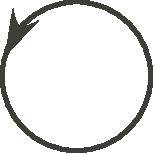
\includegraphics[width=.8cm]{pictures/unknot}}\Bigr\rangle=-\frac{\alpha+\gamma}{\beta}~.
\ee
To determine the coefficients $\alpha,\beta,\gamma$, we need to use the braiding operator $B$. It is easy to see that
$$
B L_+ =L_0~, \qquad B^2 L_+ =L_-~.
$$
Also, the braiding matrix is a 2-by-2 matrix so that it is
$$
B^{2}-(\Tr B) B+(\det B)=0~.
$$
Therefore, we have
$$
L_- -(\Tr B) L_0+(\det B)L_+=0~.
$$
The braiding matrix can be computed by representation theory
$$
B=\begin{pmatrix}
q &0 \\ 0&-q^3
\end{pmatrix}
$$
which gives the skein relation \eqref{skein-relation}. Therefore, the Jones polynomial of the unknot \eqref{unknot} is
\be
\Bigl\langle \raisebox{-.3cm}{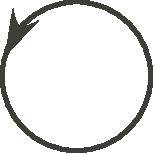
\includegraphics[width=.8cm]{pictures/unknot}}\Bigr\rangle=\frac{q^2-q^{-2}}{q-q^{-1}}=[2]_{q}~.
\ee




\subsubsection*{TQFT axiom}
Motivated by the work of Witten, Atiyah gives the axiom of topological quantum field theory \cite{atiyah1988topological}.
To each compact oriented $d$-dimensional smooth manifold $\Sigma$
without boundary one associates a finite-dimensional
vector space $\cH_{\Sigma}$. A compact oriented $(d+1)$-dimensional smooth manifold
$M$ with $\partial M= \Sigma$ determines a vector $Z(M) \in \cH_{\Sigma}$.

\begin{enumerate}
\item If $-\Sigma$ is the surface with orientation reversed, then we associate the dual vector space $\cH_{-\Sigma}=\cH_{\Sigma}^{*}$.
\item For disjoint union $\Sigma_{1} \cup \Sigma_{2}$, we have $\cH_{\Sigma_{1}} \otimes \cH_{\Sigma_{2}}$. Therefore, for $\partial M=\left(-\Sigma_{1}\right) \cup \Sigma_{2}$, a vector $Z(M) \in \cH_{\Sigma_{1}}^* \otimes \cH_{\Sigma_{2}}$ is indeed a linear map $Z(M):\cH_{\Sigma_{1}}\to \cH_{\Sigma_{2}}$.
\item For the composition of cobordisms $\partial M_{1}=\left(-\Sigma_{1}\right) \cup \Sigma_{2}$, $\partial M_{2}=\left(-\Sigma_{2}\right) \cup \Sigma_{3}$, we have
$$Z\left(M_{1} \cup M_{2}\right)=Z\left(M_{2}\right) \cdot Z\left(M_{1}\right)$$
where $Z\left(M_{1}\right): \cH_{\Sigma_{1}} \rightarrow \cH_{\Sigma_{2}}$ and $Z\left(M_{2}\right): \cH_{\Sigma_{2}} \rightarrow \cH_{\Sigma_{3}}$
\item For an empty set, we have $\cH_{\emptyset}=\mathbb{C}$.
\item $I=[0.1]$ an interval, then $Z(\Sigma \times I)$ is the identity map as a linear transformation $\cH_{\Sigma}$. Consequently, we have
$$
\Tr \Id= Z(\Sigma \times S^1)= \dim \cH_{\Sigma}~.
$$
\end{enumerate}



\end{document}
